\documentclass[tikz, svgnames]{standalone}

\usepackage{mathtools}

\let\Im\relax
\DeclareMathOperator{\Im}{Im}
\let\Re\relax
\DeclareMathOperator{\Re}{Re}

\def\xr{4} \def\yr{4}

\begin{document}
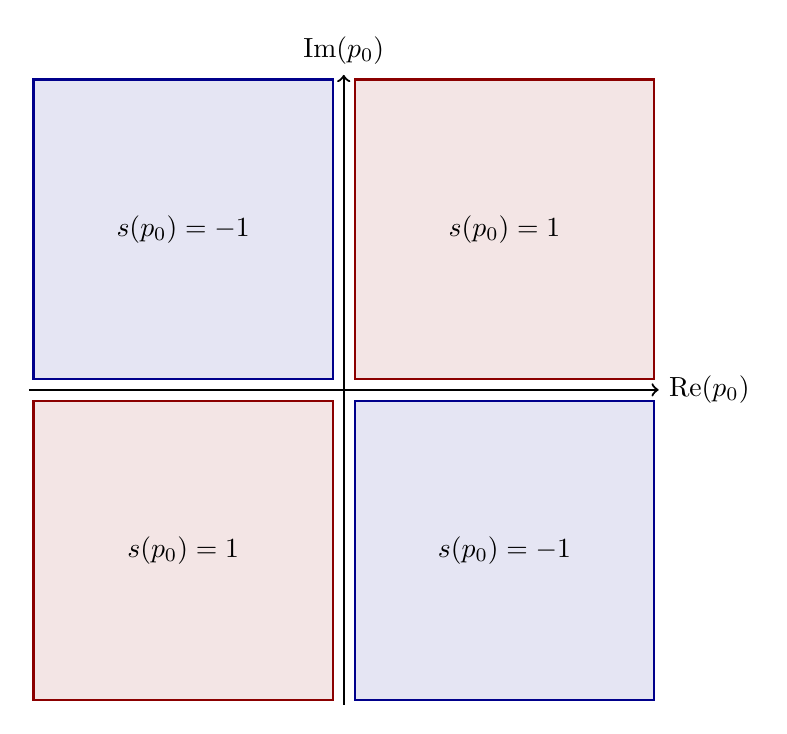
\begin{tikzpicture}[thick]

  % Axes
  \draw[->] (-\xr, 0) -- (\xr, 0) node [right] {$\Re(p_0)$};
  \draw[->] (0, -\yr) -- (0, \yr) node[above] {$\Im(p_0)$};

  % Squares
  \draw[xshift=4, yshift=4, scale=0.95, DarkRed, fill=DarkRed!10] (0, 0) rectangle (\xr, \yr) node[black, midway] {$s(p_0) = 1$};
  \draw[xshift=-4, yshift=4, scale=0.95, DarkBlue, fill=DarkBlue!10] (0, 0) rectangle (-\xr, \yr) node[black, midway] {$s(p_0) = -1$};
  \draw[xshift=-4, yshift=-4, scale=0.95, DarkRed, fill=DarkRed!10] (0, 0) rectangle (-\xr, -\yr) node[black, midway] {$s(p_0) = 1$};
  \draw[xshift=4, yshift=-4, scale=0.95, DarkBlue, fill=DarkBlue!10] (0, 0) rectangle (\xr, -\yr) node[black, midway] {$s(p_0) = -1$};

\end{tikzpicture}
\end{document}
